 \chapter{Requirements and Analysis}

With the introduction to Manta Flow platform covered, we now have enough information required to understand and analyze the problem of embedded code analysis in its context. In this chapter we will first present a motivational example for embedded code analysis, discuss requirements set by Manta Flow stakeholders, analyze multiple data technologies that support embedded code and finally we will analyze how to integrate embedded code analysis into scanners.

\section{Purpose of embedded code analysis}

We have already briefly explained what embedded code is and why it makes sense to analyze it in Manta Flow. Let us present an example that will support this explanation. It can help us build a better understanding of the motivation and illustrate some of the challenges that we need to overcome.
\par
This example is based on a real customer inquiry. A company has decided to move a part of their systems from self-hosted solution to a cloud-based solution. The migrated system cleans, pre-processes and combines data from multiple sources to create a high-quality data source for business analyses. They decided to use AWS (Amazon Web Services) as their cloud service provider. The new pipeline uses Amazon S3, Amazon Redshift and AWS Glue. Amazon S3 is a cloud object storage which is often used to store files used by other services. Amazon Redshift is a data warehousing service based on PostgreSQL database and optimized for scalability and big data processing. AWS Glue is an ETL tool which we have already introduced and will work with later in the thesis. The transformation jobs in AWS Glue are written in Python. The pipeline roughly follows these steps~(shown in figure~\ref{fig:pipelineExample}):
\begin{enumerate}
    \item Files containing raw unprocessed data are uploaded to Amazon S3.
    \item An AWS Glue job is executed which reads these files and normalizes the data - fills empty values, normalizes column names, etc. and stores it in a common data format under curated files on Amazon S3.
    \item Other AWS Glue jobs can be executed which read one or several curated files, combine the data and store it in a table in Amazon Redshift.
    \item Amazon Redshift is the final destination of this data pipeline. It is then used as a data source for visualisations and analytics.
\end{enumerate}

\begin{figure}[ht]\centering
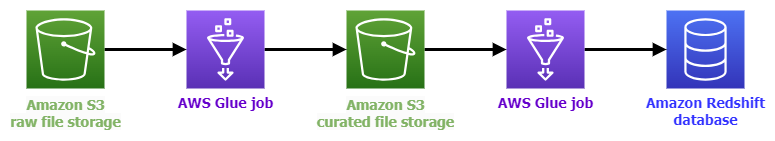
\includegraphics[width=1.0\textwidth]{img/pipeline_example.png}
\caption{A diagram of data flows in the pipeline}
\label{fig:pipelineExample}
\end{figure}

\par
Projects of this magnitude may take several months to complete, involve tens of employees who spend hundreds to thousands of man-days working on it. At this scale, it is important to keep a good overview on the progress to complete the project successfully. The customer has previously used Manta Flow to analyze different systems and would like to use it on this project as well. They would like to use it initially to watch the migration process and ensure that the new pipeline behaves correctly and no processes have been missed. After the project is over, they would like to continue using it to help with maintenance and problem resolution. The final dataset is a source for important financial and customer behavior analyses which directly impact many business decisions, so it is critical that the data is assembled correctly and data lineage visualization can help in that effort.
\par
How can data lineage analysis of embedded code help the customer? The pipeline consists of two data storage technologies, Amazon S3 and Amazon Redshift. They are only locations where data is stored. In order to find out how, for example, values in column \textit{average\_price} in table \textit{Sales} are computed, we must look into one of the AWS Glue jobs. An AWS Glue job runs a Python or Scala script on Apache Spark engine, which is a popular engine for large-scale data analytics. Therefore to provide the data lineage graph, we must run data flow analysis of the job's embedded code. When the analysis is successful, to find out how a value is computed we simply need to click on it in the visualized graph and follow the lineage. Without it we would have to locate the job manually, which might not be easy among 10s or 100s of them.

%%%%%% TODO
% 1 vziat requirements a rozpisat ich ako poziadavky zo strany Manty, zanalyzovat a vysvetlit ich
% 2 rozsirit analyzu technologii, pridat nejake priklady. 
% 3 Nasleduje analyza, ze to bude nejaka service atd, kde priblizime, ako funguje query service a porovnanie, co je stejne, co je odlisne a co by slo vyuzit
% Na konci kapitoly musi byt jasne, co ideme robit

\section{Requirements from Manta}

As this work has been assigned by and developed in cooperation with Manta Tools company which develops Manta Flow, they have set certain requirements that the final solution should fulfill. In this section we will first, state a requirement and then we will follow-up with a discussion about its motivation and implications.

\subsection{Functional requirements}

These requirements define what the solution nedds to and needs not to do.

\subsubsection{Embedded code analysis}

\textit{Provided a code script (string/file, not important implementation detail) and configuration, the service analyzes the script and delivers lineage graph for that script}. This requirement is pretty straight-forward, it describes what is to be delivered.
\par
Firstly, we shall discuss why a service is required. \textit{Service} is a wide term and its concrete meaning depends on the context. There is already \textit{Dataflow Query Service} in Manta Flow which handles analysis of embedded database queries and scripts. In its core it is a Java bean (a class that encapsulates one or more objects into a single standardized object) which uses specific parts of database scanners to process the queries. It is called a service, because it is a reusable component (a bean) that can be used by any scanner and it provides its services through a standardized interface with a specific input and output. The solution described in this work, Embedded Code Service, is in many ways similar to Dataflow Query Service so it is expected to be used in a similar way.
\par
The service shall accept embedded code as one of its inputs. That is different from how scanners in Manta Flow usually work, because they collect their inputs themselves. It shall also accept configuration. What will it be used for? Scanners in Manta Flow have many configurable properties which influence their execution, users may modify them in \textit{Manta Admin UI}. It must be possible to configure how embedded code is analyzed as well. Additionally, from the description of embedded code we know that it is executed in the environment provided by the data technology. This environment can differ from standard runtime environment, so any differences, e.g. environment variables, pre-included libraries, need to be passed to the service in some way - in the configuration.
\par
The last part of this requirement describes that the service shall perform data flow analysis of the input and provide the data lineage graph on the output for further processing. Contrary to the standard scanner workflow, the Manta graph is not uploaded to \textit{Manta Flow Server}, but returned as return value.

\subsubsection{Graph merging}

\textit{The service can merge the lineage graph with the lineage graph of parent data technology when provided a node to be merged with}. This requirement extends the previous one and describes what is to be done with the output.
\par
Each scanner produces one Manta graph for one input. When it uses a service to process a part of the input, which creates other graphs, they need to be merged. The merge operation is not a trivial process, so it shall be the responsibility of the service to implement it. The benefits are easy to see, no need to implement it each time the service is used across different scanners, which improves maintainability of the solution and also there is no need to understand it outside of the service. The developers may simply use the service interface to merge the results.

\subsubsection{Multi-purpose service}

\textit{The service can support multiple parent data technologies - technologies that support usage of user-defined embedded code}. This requirement states that the service is multi-purpose, so there is one such service available instead of there being many services for processing embedded code in each data technology.

\subsection{Qualitative (non-functional) requirements}

On top of the definition of functionality of the solution, there are also some requirements defining its qualities.

\subsubsection{Optimized for scanning}

\textit{The service should be optimized to handle tens to hundreds of scripts for a specific combination of technology-scanner in one analysis - the limitation should be the speed of the scanner, not the speed of the service}. In general, the service can be expected to be used multiple times by one scanner when it processes one connection, there may be several embedded code scripts. It is important to keep that in mind in its design. The service is intended to facilitate data lineage scanning and most of its execution time should be spent doing so. All other work that the service needs to do shall be reasonably optimized so that this overhead does not add up to a lot when it is called multiple times. This requirement does not intend to include specific scanner optimizations that can be made to improve the overall execution time of the service as they shall be evaluated after this solution is implemented and are outside of the scope of this work.

\subsubsection{Extendibility}

\textit{Extending supported data technologies should be simple, adding a new technology should only include collecting its configuration in the technology scanner and implementing this configuration in embedded code service}. It is expected that the list of the scanners that use the service will grow in time based on customer requirements and available development capacity. The service shall be designed in a way that promotes extendibility so that the effort required to add support for new data technology is minimised. This can be done by splitting the code base to a common and a specific part so that it is obvious what needs to be added or modified in order to extend the service.

\subsubsection{Code reuse}

\textit{Maximize code reuse. Reuse the existing scanners and logic}. Scanners for analyzing programming language source code are very complex. We shall use the existing scanners and make only the necessary modifications to be able to analyze embedded code. Developing one scanner for analyzing both applications and embedded code is a preferred way from resource allocation perspective.

\subsubsection{Code duplication}

\textit{Minimize code duplication, no logic should be written on more than one place}. One of the purposes of the service is to hide repeating blocks of code that are tied with its use. Deduplication improves maintainability, because when a process needs to be changed, it only needs to be changed in one place instead of in multiple location. One of the examples of such practice is graph merging logic mention in one of the previous requirements.

%%----- SECTION -----%%
\section{Source technology analysis}

Before we dive further into the analysis, we need to examine which source data technologies, whether currently supported by Manta Flow or planned, support embedded code. Limiting to these technologies is driven by business requirements, it does not make sense to support analysis of embedded code in a data technology that is not used by any current or prospective customer. This overview will give us a better understanding of the range of embedded code use-cases, their similarities and differences.

\subsubsection{Hive}
Hive is a distributed data warehouse system that allows users to read, write and manage big volumes of data using SQL. Starting from version 0.13.0, it supports writing user-defined functions in Java which accept parameters and return a value. The function is implemented by a class that extends a Hive \texttt{UDF} base class. These base classes define methods that shall be implemented by the function and will be invoked in specific order on SQL query execution. This class is then supposed to be packaged in a JAR referenced by a URI from which it will be loaded into the environment~\cite{hive}. An example of a user-defined function implementation that turns a string into lower case can be seen in figure~\ref{fig:hiveScript}.

\begin{figure}[ht]
\begin{lstlisting}[language=Java]
package com.microsoft.examples;

import org.apache.hadoop.hive.ql.exec.Description;
import org.apache.hadoop.hive.ql.exec.UDF;
import org.apache.hadoop.io.*;

// Description of the UDF
@Description(
    name="ExampleUDF",
    value="returns a lower case version of the input string.",
    extended="select ExampleUDF(deviceplatform) from hivesampletable limit 10;"
)
public class ExampleUDF extends UDF {
    // Accept a string input
    public String evaluate(String input) {
        // If the value is null, return a null
        if(input == null)
            return null;
        // Lowercase the input string and return it
        return input.toLowerCase();
    }
}
\end{lstlisting}
\caption{An example of a Hive user-defined function written in Java~\cite{hiveudfexample}}
\label{fig:hiveScript}
\end{figure}

\subsubsection{Microsoft SQL Server}
Microsoft SQL Server enables users to implement stored procedures, triggers, user-defined types, user-defined functions (scalar and table valued), and user-defined aggregate functions using any .NET Framework language, including Microsoft Visual Basic .NET and Microsoft Visual C\#. They can be implemented by arbitrary classes and methods as long as they are properly annotated. These annotations facilitate the lookup and binding between SQL Server and embedded code. Compiled code is distributed in DLL and loaded into environment using SQL syntax~\cite{mssql}.

\subsubsection{SQL Server Integration Services (SSIS)}
SSIS is a platform for data integration and transformation solutions. It provides graphical tools for building ETL workflows, but it is also possible to create custom objects programmatically in C\# or Visual Basic. These include tasks, connection managers, log providers, enumerators and data flow components. Implementations of custom objects are expected to extend one of the base classes provided by SSIS, to override required methods and to use proper attributes. These objects are then distributed as a compiled class library. This is a similar approach as that of MSSQL~\cite{ssis}.
\par
In an example shown in figure~\ref{fig:cSharpScript}, a script component is defined as a class which inherits from the \texttt{UserComponent} base class provided by SSIS. The \texttt{CreateNewOutputRows} method is overridden to implement the desired logic. Within it we can access the input column values using the \texttt{Variables} object, which provides access to the input columns. In this example, the value of the first input column (MyInputColumn) is retrieved and stored in the \texttt{inputColumnValue} variable. Next, a transformation is performed on the input column value (in this case, converting it to uppercase), and the result is stored in the \texttt{outputColumnValue} variable. Finally, a new output row is added using the \texttt{OutputBuffer} object, and the transformed value is assigned to the output column (MyOutputColumn).

\begin{figure}[ht]
\begin{lstlisting}[language=csh]
using System;
using System.Data;
using Microsoft.SqlServer.Dts.Pipeline.Wrapper;
using Microsoft.SqlServer.Dts.Runtime.Wrapper;

[Microsoft.SqlServer.Dts.Pipeline.SSISScriptComponentEntryPointAttribute]
public class ScriptMain : UserComponent
{
    public override void CreateNewOutputRows()
    {
        // Accessing input column values
        string inputColumnValue = string.Empty;
        if (Variables.MyInputColumn != null && Variables.MyInputColumn.Length > 0)
        {
            inputColumnValue = Variables.MyInputColumn[0].ToString();
        }

        // Performing some transformation on the input column value
        string outputColumnValue = inputColumnValue.ToUpper();

        // Creating new output rows
        Output0Buffer.AddRow();
        Output0Buffer.MyOutputColumn = outputColumnValue;
    }
}
\end{lstlisting}
\caption{An example of an SSIS script component written in C\#}
\label{fig:cSharpScript}
\end{figure}

\subsubsection{PostgreSQL}
By default, PostgreSQL supports functions written in C, but theoretically users may use any language, as long as it can be made compatible with C, e.g. C++. However, that is often difficult due to different calling conventions, so its safe to assume C language is used. The function definitions are supposed to use macros from \texttt{postgres.h} header file, but otherwise are common C functions. The code is compiled and dynamically loaded into the environment using SQL. There is currently no plan to support analyzing C language, so this data technology is mentioned only for completeness~\cite{postgresql}.

\subsubsection{Snowflake}
Snowflake Data Cloud is a cloud-based data storage and analytics service. It is common to use SQL to interact with data in Snowflake and embedded code is integrated in a similar way in the form of functions and stored procedures. Apart from SQL, these can be written in multiple programming languages - Java, Scala, JavaScript or Python. Each language used has (slightly) different capabilities and requirements. In case of JavaScript, it can be used to execute SQL statements and interact with the result to provide a return value. Java, Scala and Python scripts have to contain a function or a method with the first argument of type \texttt{Session} from Snowflake's Snowpark library. This argument will be populated by Snowflake when the procedure/function is invoked and is used for interaction with Snowflake platform~\cite{snowflake}.

\begin{figure}[ht]
\begin{lstlisting}[language=SQL]
CREATE OR REPLACE PROCEDURE my_stored_procedure(param1 STRING, param2 INT)
RETURNS STRING
LANGUAGE PYTHON
AS
$$
    import snowpark as sp

    @sp.session
    def my_snowpark_function(session):
        # Create a DataFrame using the provided parameters
        df = session.range(0, param2).select(sp.lit(param1).alias('Value'))
        
        # Perform some transformations on the DataFrame
        transformed_df = df.withColumn('Length', sp.length(df['Value']))
        
        # Convert the transformed DataFrame to a Pandas DataFrame
        pandas_df = transformed_df.toPandas()
        
        # Generate a summary string
        summary = pandas_df.describe().to_string()
        
        return summary
    
    # Call the Snowpark function with the provided parameters
    return my_snowpark_function(param1, param2)
$$;
\end{lstlisting}
\caption{An example of a Snowflake stored procedure written in Python}
\label{fig:snowflakeScript}
\end{figure}

\par
In an example shown in figure~\ref{fig:snowflakeScript}, we are creating a stored procedure written in Python that takes two parameters, a string and an integer. The body of the stored procedure contains a Python function named \texttt{my\_snowpark\_function}. This function uses the Snowpark session decorator to establish a session with Snowflake. Within the function, we create a DataFrame and perform some transformations on it. In this example, we add a new column \textit{Length} that calculates the length of the \textit{Value} column. Next, we convert the transformed DataFrame to a Pandas DataFrame and generate a summary string from it. Finally, the stored procedure calls the \texttt{my\_snowpark\_function} with the provided parameters and returns the summary string.

\subsubsection{Databricks}
Databricks is a web-based data platform that combines data warehouses and data lakes with analytics build on Apache Spark and IPython-style notebooks. These notebooks are interactive computational environments. They consist of a sequential combination of cells which may contain rich text, embedded code, data visualization etc. Embedded code cells may be written in Python, Scala, SQL or R and it is possible to combine cells written in different languages in one notebook. During a notebook execution, cells written in the same language are executed in the same environment and may interact with other language environments using shared context of Apache Spark~\cite{databricks}.
\par
Let us have a notebook consisting of a Python cell (shown if figure~\ref{fig:pythonDatabricks}) and an SQL cell (shown in figure~\ref{fig:sqlDatabricks}). The Python cell sets the value of the shared variable which is then printed to the standard output. The SQL cell showcases how to access the shared variable within an SQL statement using the \$ symbol. In this example, we update the value of column1 based on the value stored in the shared variable.

\begin{figure}[ht]
\begin{lstlisting}[language=Python]
# Define a shared variable
dbutils.shared.notebook.set("my_shared_variable", "Hello, Databricks!")

# Access the shared variable
shared_value = dbutils.shared.notebook.get("my_shared_variable")
print(shared_value)
\end{lstlisting}
\caption{Python cell of a Databricks notebook}
\label{fig:pythonDatabricks}
\end{figure}

\begin{figure}[ht]
\begin{lstlisting}[language=SQL]
-- Update a table using the shared variable in SQL
UPDATE my_table
SET column1 = $my_shared_variable
WHERE condition;
\end{lstlisting}
\caption{SQL cell of a Databricks notebook}
\label{fig:sqlDatabricks}
\end{figure}

\subsubsection{AWS Glue}
AWS Glue is a fully managed ETL service provided by Amazon Web Services (AWS). It simplifies the process of preparing and loading data for analytics, data warehousing, and other data-related tasks. With AWS Glue, you can create and schedule ETL jobs to automate the data transformation and loading process. It handles the execution, monitoring and orchestration of these jobs. ETL jobs leverage the underlying Apache Spark framework for distributed data processing. Each job is defined by a script written in Python or Scala. This script can be written manually or the job's workflow is built in an interactive GUI and the code is generated automatically. Compared to other data technologies, AWS Glue is built entirely on embedded code. That means that each ETL job is executed entirely by a single Python/Scala script as opposed to only parts of data operations in other data technologies~\cite{awsglueintro}.
\par
The example in figure~\ref{fig:embeddedScript} show code of an ETL job that performs data processing and transformation, combining data from different sources and storing the result in an S3 bucket. Firstly, we read data from a specified database and tables into dynamic frames on which we perform data transformations. The \texttt{products} frame is modified by dropping certain fields and renaming one. Multiple joins are applied to the frames, first between \texttt{products} and \texttt{purchases}, and then between the resulting frame and \texttt{suppliers}. The resulting frame is written to an S3 location in the parquet format.

\begin{figure}[ht]
\begin{lstlisting}[language=Python]
import sys
from awsglue.transforms import Join
from pyspark.context import SparkContext
from awsglue.context import GlueContext

glueContext = GlueContext(SparkContext.getOrCreate())

db_name = "main_db"
output_dir = "s3://glue-example/output/supply_chain"

# Create dynamic frames
products = glueContext.create_dynamic_frame.from_catalog(database=db_name, table_name="products_json")
purchases = glueContext.create_dynamic_frame.from_catalog(database=db_name, table_name="purchases_json")
suppliers = glueContext.create_dynamic_frame.from_catalog(database=db_name, table_name="suppliers_json")

# Keep the fields we need and rename some
products = products.drop_fields(['color', 'identification']).rename_field('name', 'product_name')

# Join the frames
result = Join.apply(Join.apply(products, purchases, 'id_product', 'product_id'), suppliers, 'supplier_id', 'id_supplier')

# Write out the frame into parquet file
glueContext.write_dynamic_frame.from_options(frame = result, connection_type = "s3", connection_options = {"path": output_dir}, format = "parquet")
\end{lstlisting}
\caption{An example of an embedded script in AWS Glue}
\label{fig:embeddedScript}
\end{figure}

\subsubsection{Other data technologies}
Besides the data technologies already described, there are others that provide embedded code integration and are supported in Manta Flow. These follow similar principles as some that were already described before, so we will not cover them in detail. However, we list them below for completeness:
\begin{itemize}
    \item Talend supports extending the functionalities of a Talend Job using custom Java commands~\cite{talend}.
    \item Google BigQuery supports defining functions written in JavaScript~\cite{bigquery}.
    \item StreamSets allows creating custom StreamSets processors in Java~\cite{streamsets}.
    \item Informatica supports creating custom components with Java~\cite{informatica}.
    \item Azure Data Factory supports creating Custom activity with own data movement or transformation logic in C\# that can be added to a pipeline~\cite{adf}.
    \item SAS supports running Python statements within a SAS session~\cite{sas}. Additionally, there are multiple Python packages for interacting with SAS from Python.
\end{itemize}

\subsection{Embedded code usage philosophy}
Based on the description of embedded code usages, we can observe a few repeating patterns. These will help us design embedded code service.
\par
We can see that database systems use embedded code in the form of user-defined functions or stored procedures. They can then be invoked as a part of an SQL query or an SQL script. They often return a value and may receive arguments.
\par
Another common use-case is to define a custom transformation or a task in an ETL workflow. The details of this use-case vary more than those in database systems but in general they implement a specific interface which functions are invoked in a pre-determined order by the data technology.
\par
Next observation relies to the programming language being used. Most often we can see Java or Scala, .NET languages (mainly C\# or Visual Basic) and Python. Sometimes also JavaScript is used and there is one case of R and C, but we shall ignore them as there isn't currently a language scanner implemented in Manta Flow for them.
\par
In compiled static-typed languages (Java and C\#), it is common to tag the classes that shall be used as embedded code and require a rigid interface, either by extending a base class or using annotations. The code is distributed in compiled form and loaded dynamically. Interaction with the data technology is facilitated through an object that is provided as a method argument or a property of a base class.
\par
As Python is interpreted and not compiled, it is possible to inject the embedded code into a different code to create a new script. That allows use-cases where some code is executed before embedded code which defines some variables, functions, classes etc. The embedded code may then directly read these identifiers without having to declare them, which is used to provide interface for interacting with data technology. To successfully analyze such approach, it is important to understand and simulate these assignments.




